% !TEX root = ../DP_Vik_Tomas_2013.tex
\chapter{Wireframe}
\label{chp:wireframe}
Díky prostorové náročnosti se kompletní dokumentace vytvoření drátěného modelu nachází zde v příloze.

\section{Hlavní ovládací prvky}
\label{sec:hlavni-ovladaci-prvky}
Hlavní ovládací prvky dokáží spouštět akce popsané v kapitole \ref{sec:hlavni-akce}. Tyto prvky musí být umístěny na každé stránce, a proto se nachází v tzv. layoutu webové aplikace. Návrh layoutu výsledné aplikace se nachází na obrázku \ref{fig:mock-layout}.

\begin{figure}[htb]
\begin{center}
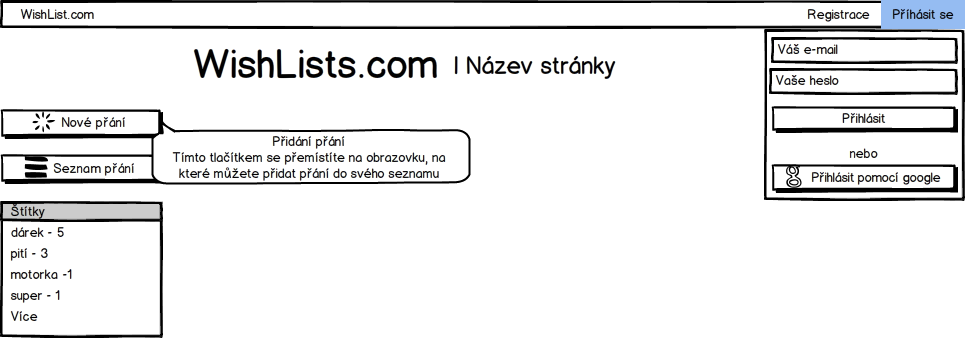
\includegraphics[width=130mm]{./pictures/mock/layout.png}
\caption{Drátěný model layoutu stránky.}
\label{fig:mock-layout}
\end{center}
\end{figure}

V návrhu layoutu je jasně vidět panel umístěný v horní časti stránky, který obsahuje prvky pro přihlášení a odkaz na domovskou stránku. Dále je v horní části stránky název aplikace, který je zároveň také odkazem na domovskou stránku. V levé části se nachází navigace, která se skládá z odkazů na přechod na přidání přání a seznam přání a ze seznamu všech štítků, u kterých je zároveň uvedeno, kolik přání je u nich obsaženo.

\section{Hlavní obrazovky}
Dále budou popsány obrazovky, které zabírají celou stránku. Tyto stránky vždy obsahují výše zmíněné \nameref{sec:hlavni-ovladaci-prvky}. Všechny obrazovky kromě \ref{sc-01} jsou navrhnuty z pohledu nepřihlášeného uživatele\footnote{Hlavní ovládací prvky umožňují přihlášení a registraci namísto odhlášení.}.

\subsection{\ref{sc-01}}
Toto je stránka, která se zobrazí uživateli ihned po jeho přihlášení do aplikace. Zároveň ho na ní přesunou oba odkazy umístěné v hlavních ovládacích prvcích. Na této stránce bude uživateli zobrazeno maximálně pět přání. Výběr přání bude proveden na základě nejprudší změny ceny (a to ať už zlevnění, nebo zdražení produktu). Stránka je na obrázku \ref{fig:uvodni-prihlaseny-uzivatel}. Na této obrazovce není možné přání přesouvat, protože zde nejsou seřazena podle priority.

\begin{figure}[htb]
\begin{center}
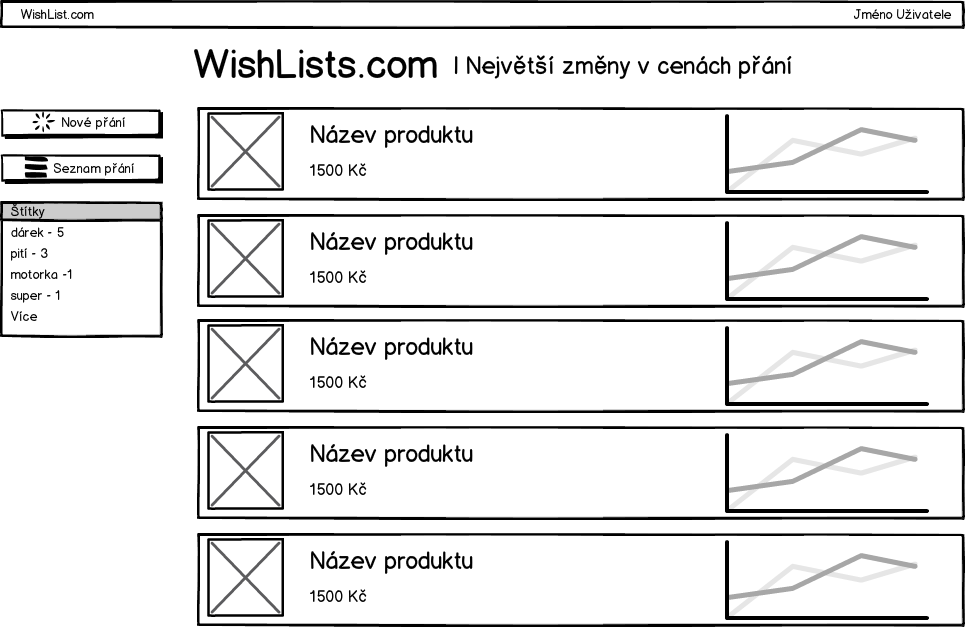
\includegraphics[width=130mm]{./pictures/mock/uvodni-prihlaseny-uzivatel.png}
\caption{\ref{sc-01}}
\label{fig:uvodni-prihlaseny-uzivatel}
\end{center}
\end{figure}

\subsection{\ref{sc-02}}
Na tuto stránku uživatel přejde, pokud zvolí hlavní ovládací prvek přidat přání. Zde je uživateli umožněno vyhledat produkt podle jeho názvu. Návrh je na obrázku \ref{fig:vyhledavani}. V centru stránky je velké vstupní pole pro zadání názvu produktu.

\begin{figure}[htb]
\begin{center}
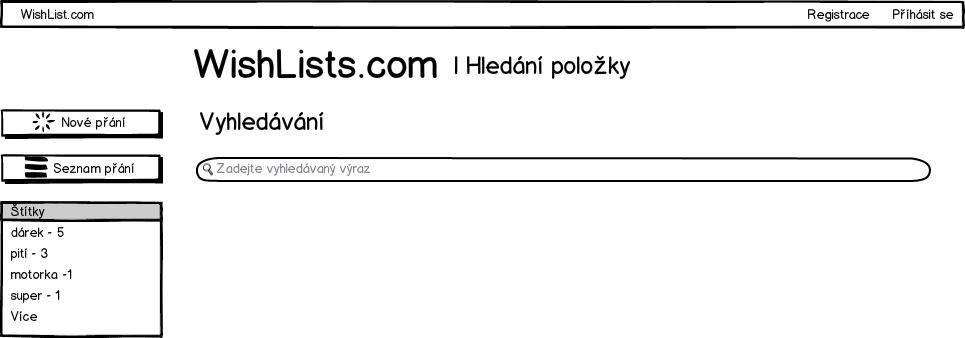
\includegraphics[width=130mm]{./pictures/mock/vyhledavani.png}
\caption{\ref{sc-02}}
\label{fig:vyhledavani}
\end{center}
\end{figure}

\subsection{\ref{sc-03}}
Po zadání hledaného výrazu zobrazí aplikace uživateli výsledky. Pokud nenajde žádný výsledek, zobrazí zprávu, která o tom uživatele informuje. Návrh obrazovky je na obrázku \ref{fig:vysledky-hledani}

U každého výsledku je ukázán obrázek produktu, jeho celý název, popisek, rozmezí cen, ve kterém se produkt pohybuje a tlačítko pro vytvoření přání. Ve skutečnosti celý výsledek reaguje na kliknutí myši. Tlačítko je u výsledku primárně, aby uživatel věděl, co se s výsledkem dělá.

\begin{figure}[htb]
\begin{center}
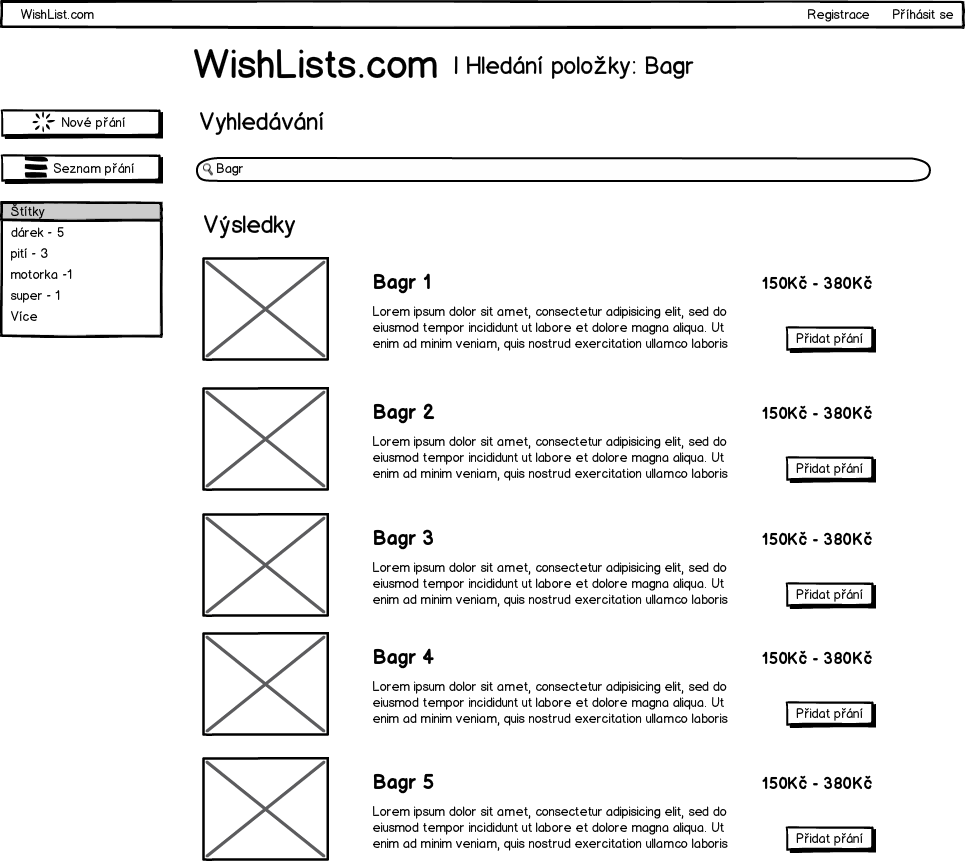
\includegraphics[width=130mm]{./pictures/mock/vysledky-hledani.png}
\caption{\ref{sc-03}}
\label{fig:vysledky-hledani}
\end{center}
\end{figure}

\subsection{\ref{sc-11}}
\label{sec:wireframe-pridani-prani}
Poté co uživatel klikne na výsledek hledání přání, bude zobrazena obrazovka pro přidání přání.  Návrh obrazovky je na obrázku \ref{fig:formular-pridani-prani}.

Na návrhu je vidět, že uživateli je zvolen obrázek pro přání, ale zároveň má možnost vybrat z miniatur pod hlavním obrázkem a kliknutím na miniauturu nahradit původní obrázek. Vizuální stránka přání je důležitá, proto zabírá celou půlku formuláře. Zároveň je ve sloupci s obrázkem zobrazen graf vývoje ceny produktu, který má 2 křivky. Jedna určuje nejnižší cenu přání a druhá cenu přání ve vybraném obchodě.

V druhé půlce je uživateli umožněno nastavit všechny informace popsané v kapitole \ref{sec:pridani-prani}. A navíc přejít přímo na stránku produktu ve vybraném obchodě pomocí tlačítka \emph{Koupit}. Toto tlačítko je neaktivní, dokud uživatel nevybere vlastní obchod.

Rychlá priorita ulehčuje uživateli práci. Oprosťuje uživatele od vnitřní datové reprezentace priority. Nechá ho vybrat ze tří možností a na základě jednoduchého algoritmu patřičně přiřadí prioritu k přání.

Uživateli se navíc zobrazí dodatečné informace (popis a technická specifikace) o produktu, aby se mohl rozhodnout, jestli je produkt opravdu to, co hledal.

\begin{figure}[htb]
\begin{center}
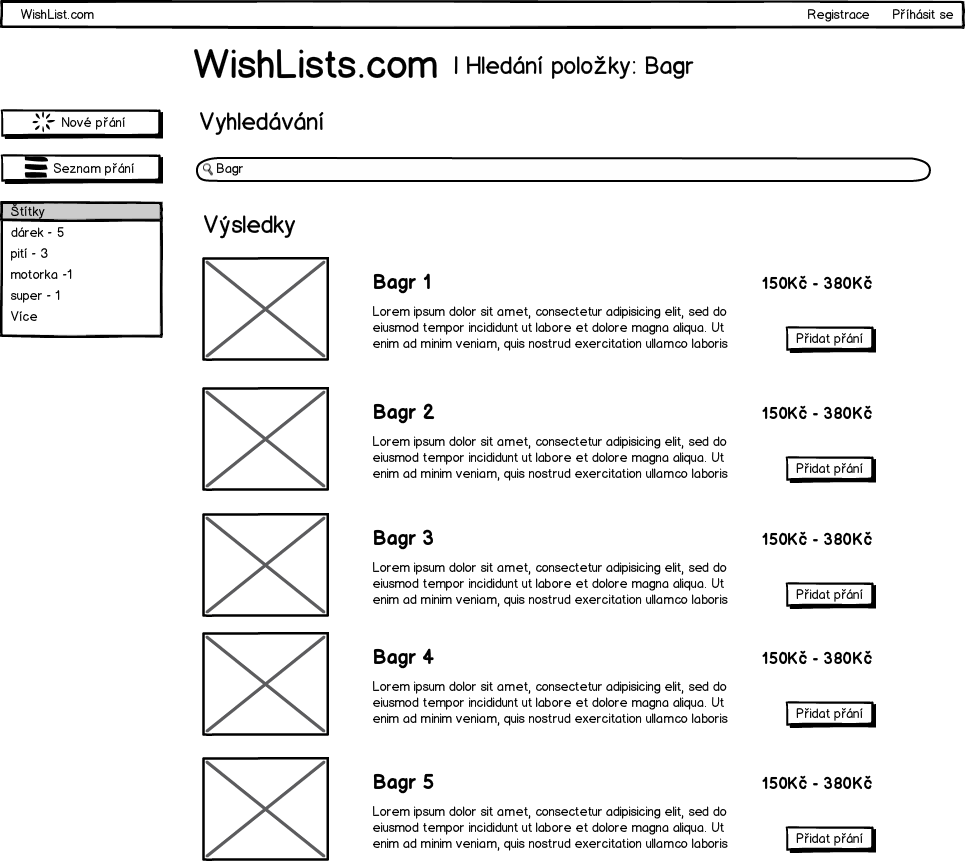
\includegraphics[width=130mm]{./pictures/mock/vysledky-hledani.png}
\caption{\ref{sc-11}}
\label{fig:formular-pridani-prani}
\end{center}
\end{figure}

\subsection{\ref{sc-04}}
\label{sec:wireframe-vsechna-prani}
Na stránce jsou uživateli zobrazena všechna jeho přání seřazena podle priority od nejvyšší po nejnižší. Návrh obrazovky je na obrázku \ref{fig:vsechna-prani}.

U každého přání je zobrazen název produktu, cena v obchodě, který je u přání přiřazen a graf aktuálního vývoje ceny.

Přání je možné přesouvat táhnutím myši a tím měnit jejich prioritu. Detail přání a případnou editaci uživatel zobrazí tlačítkem \emph{Detail}. Z tohoto výpisu je možné také přejít přímo na stránku produktu ve vybraném obchodě pomocí tlačítka \emph{Koupit}.

\begin{figure}[htb]
\begin{center}
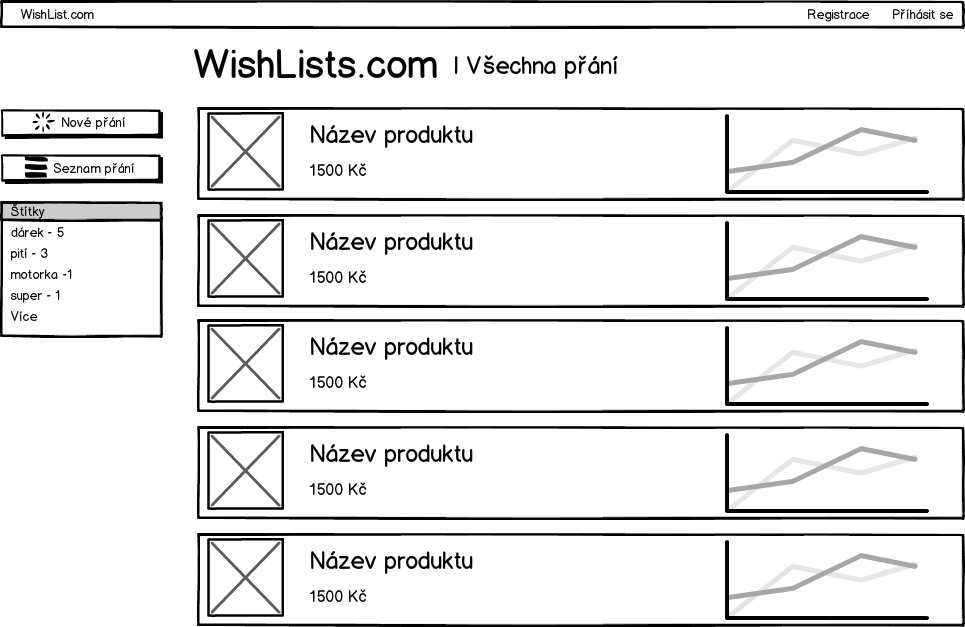
\includegraphics[width=130mm]{./pictures/mock/vsechna-prani.png}
\caption{\ref{sc-04}}
\label{fig:vsechna-prani}
\end{center}
\end{figure}

\subsection{\ref{sc-05}}
Stránka zobrazení detailu přání s možností jeho editace. Při návrhu stránky byl kladen důraz na co největší podobu se stránkou na přidání přání. Tu se totiž už uživatel musel naučit/pochopit, a proto by bylo kontraproduktivní jej nutit přemýšlet nad jinou stránkou. To odpovídá principu konzistence a standardizace\cite{molich1990improving}. Návrh obrazovky je na obrázku \ref{fig:editace-detail-prani}.

Oproti obrazovce na přidání přání byla odstraněna rychlá priorita, protože ta se teď už nastavuje na obrazovkách se seznamy přání. Přibylo tlačítko na smzání přání a důležité tlačítko, které přání označí jako splněné.

\begin{figure}[htb]
\begin{center}
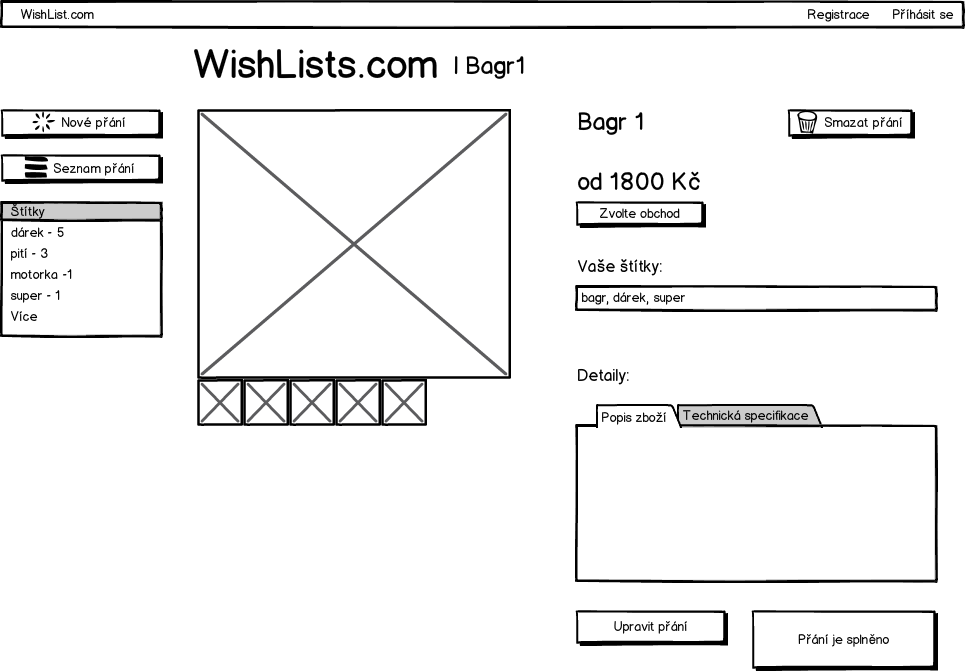
\includegraphics[width=130mm]{./pictures/mock/editace-detail-prani.png}
\caption{\ref{sc-05}}
\label{fig:editace-detail-prani}
\end{center}
\end{figure}

\subsection{\ref{sc-08}}
\label{sec:prani-podle-stitku}
Obrazovka je totožná s \ref{sc-04}, s výjimkou že jsou na ní zobrazeny pouze přání označená jedním konkrétním štítkem. Veškeré ostatní informace a funkcionalita stránky zůstavají nezměněny. Návrh obrazovky je na obrázku \ref{fig:prani-oznacena-tagem}.

\begin{figure}[htb]
\begin{center}
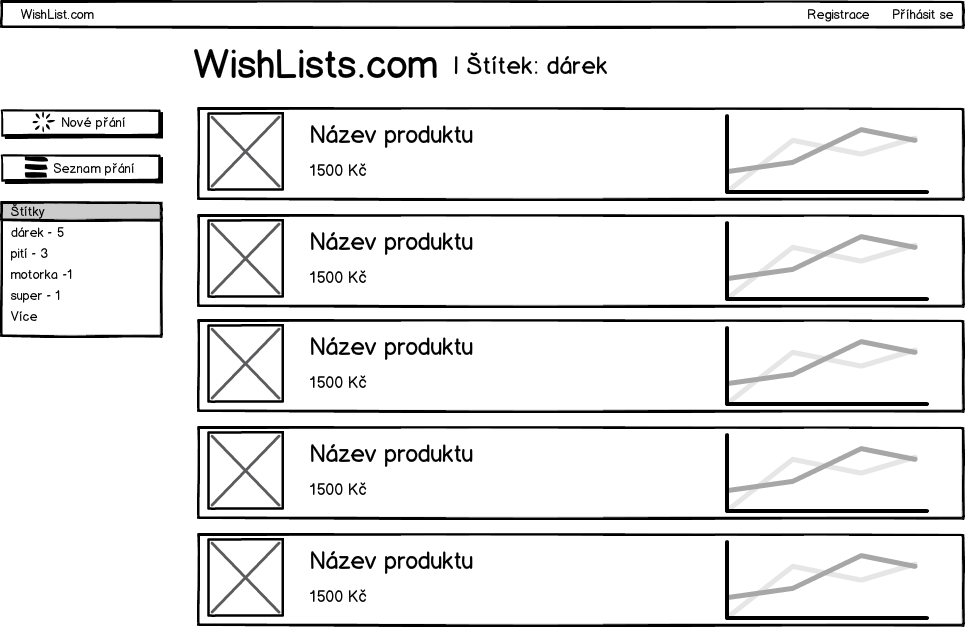
\includegraphics[width=130mm]{./pictures/mock/prani-oznacena-tagem.png}
\caption{\ref{sc-08}}
\label{fig:prani-oznacena-tagem}
\end{center}
\end{figure}

\section{Dialogy a komponenty}
Některé informace nevyžadují tolik místa, nebo je podle konvence nutné je řešit dialogem(konzistence a standardizace\cite{molich1990improving}), a proto není jejich zobrazení realizováno jako celá stránka. Namísto toho je informace zobrazená formou komponenty umístěné na hlavní ztránce, nebo dialogu zobrazeného přes libovolnou stránku.

\subsection{\ref{sc-12}}
Pokud uživatel přesáhne maxilmální počet přání (viz. sekce \ref{sec:pridani-prani}), tak mu aplikace zobrazí dialog, ve kterém má možnost zvolit jaká přání si ponechá a jaká mu smaže (obrázek \ref{fig:dialog-overflow}). V dialogu jasně vidí čítač, který ukazuje kolik přání ještě musí uživatel označit pro smazání. Přání jsou označena kliknutím.

Počet přání může uživatel překročit dvojím způsobem:
\begin{itemize}
\item Klasickým přidáním přání - uživatel jednoduše přidá přání přes limit, v tom případě se v dialogu ukáže 5 přání s nejnižší prioritou plus to nové.
\item Přidáním přání nepřihlášeného uživatele - uživatel si před přihlášením vytvořil několik přání a ta po přihlášení chce přidat do svého seznamu. V tomto případě se uživateli zobrazí stejný počet starých jako nových přání. Minimálně se ovšem starých přání zobrazí pět.
\end{itemize}

\begin{figure}[htb]
\begin{center}
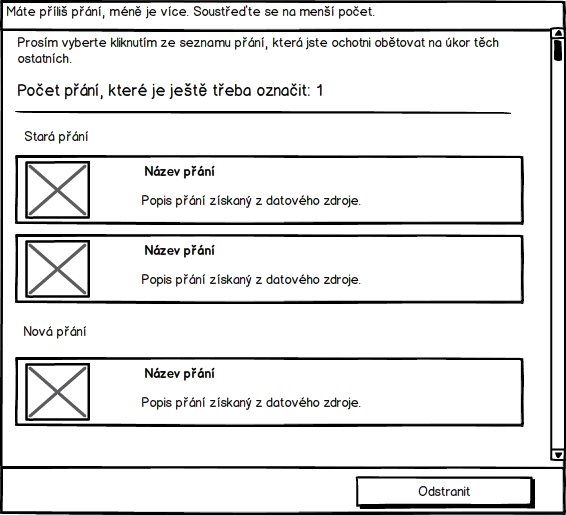
\includegraphics[width=70mm]{./pictures/mock/dialog-overflow.png}
\caption{\ref{sc-10}}
\label{fig:dialog-overflow}
\end{center}
\end{figure}

\subsection{\ref{sc-06}}
Na obrázku \ref{fig:dialog-mazani-prani} je zobrazen návrh dialogu, který se uživateli zobrazí poté, co klikne na tlačítko smazání přání. Dialog je naprosto triviální.

\begin{figure}[htb]
\begin{center}
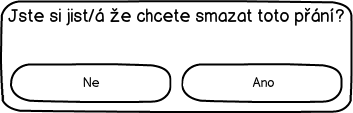
\includegraphics[width=70mm]{./pictures/mock/dialog-mazani-prani.png}
\caption{\ref{sc-08}}
\label{fig:dialog-mazani-prani}
\end{center}
\end{figure}

\subsection{\ref{sc-07}}
Komponenta je přítomna v základním layoutu a je vidět například na obrázku \ref{fig:mock-layout}. Jedná se o seznam všech štítků, kterými má uživatel označena přání. Skládá se z nadpisu komponenty, seznamu štítků a tlačítka, které umožňuje zobrazovat/skrývat další štítky. Každý šítek má u sebe zobrazeno číslo reprezentující počet přání, které jsou jím označeny. Zároveň štítek funguje jako odkaz na obrazovku s přehledem štítků (\ref{sec:prani-podle-stitku}).

Po zobrazení komponenty se v ní pro přehlednost ukazuje pouze pět nejpoužívanějších štítků. Další může uživatel zobrazit pomocí stisknutí tlačítka \emph{Více}.

\subsection{\ref{sc-09}}
Na obrázku \ref{fig:dialog-registrace} je zobrazen návrh formuláře pro registraci uživatele. Tento formulář je zobrazen v dialogu. Uživatel na něm vyplní pouze nezbytné údaje pro správnou registraci:
\begin{itemize}
\item Celé své jméno
\item E-mail
\item Heslo pro přihlášení
\end{itemize} 

\begin{figure}[htb]
\begin{center}
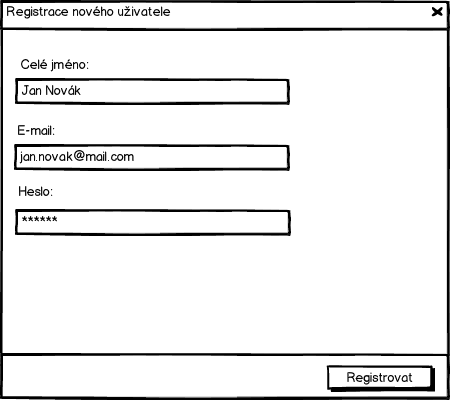
\includegraphics[width=70mm]{./pictures/mock/dialog-registrace.png}
\caption{\ref{sc-09}}
\label{fig:dialog-registrace}
\end{center}
\end{figure}

\subsection{\ref{sc-10}}
Na obrázku \ref{fig:dialog-pridani-docasnych-prani} je zobrazen návrh dialogu, na kterém má uživatel těsně po přihlášení možnost přidat ke svým přáním ta přání, která vytvořil před přihlášením.

Uživateli se zobrazí seznam všech věcí, které vytvořil před přihlášením s dotazem, zdali je chce přiřadit ke svému současnému účtu, uživatel může přijmout, nebo odmítnout.

\begin{figure}[htb]
\begin{center}
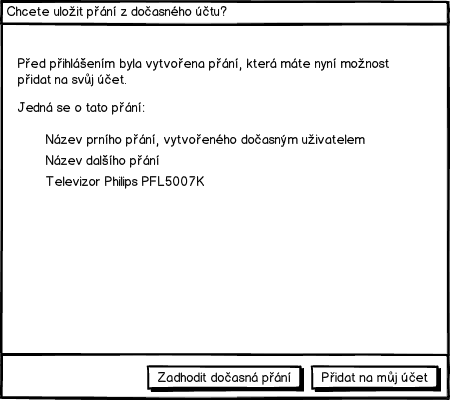
\includegraphics[width=70mm]{./pictures/mock/dialog-pridani-docasnych-prani.png}
\caption{\ref{sc-10}}
\label{fig:dialog-pridani-docasnych-prani}
\end{center}
\end{figure}
